\documentclass{standalone}
\usepackage{tikz}
\usetikzlibrary{patterns}
\usetikzlibrary{positioning}
\usetikzlibrary{patterns, positioning}
\usetikzlibrary{shapes.misc}
\usepackage[outline]{contour}
\contourlength{1.5pt} 
\usepackage[sfdefault]{ClearSans}

\begin{document}
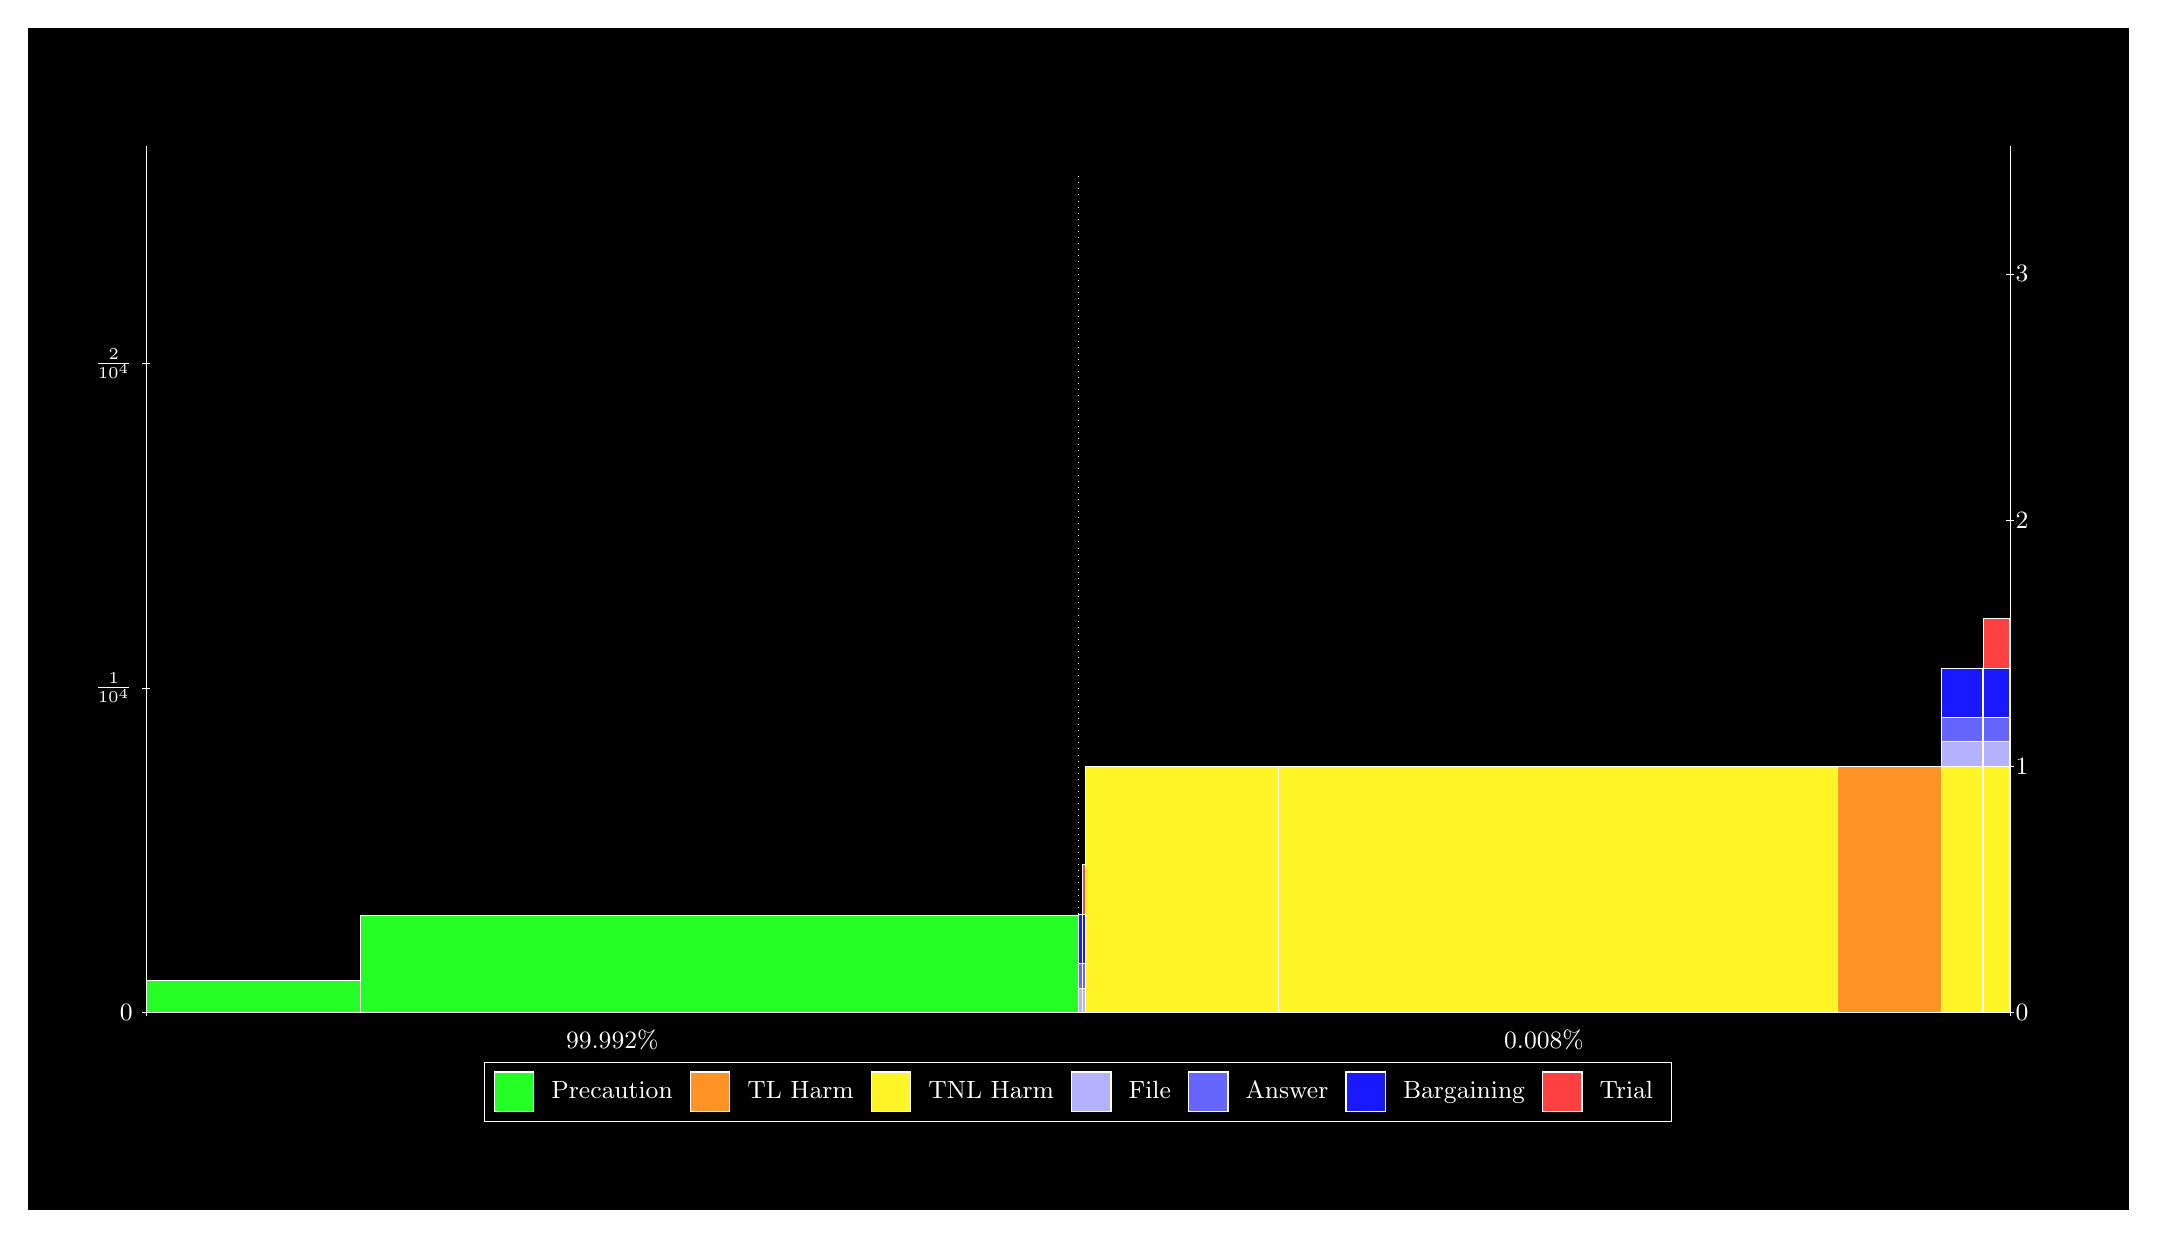
\begin{tikzpicture}
\draw[fill=black] (0,0) rectangle (26.667,15);
\draw[fill=green!85,draw=white,very thin] (1.5,2.5) rectangle (4.2218,2.9121);
\draw[fill=green!85,draw=white,very thin] (4.2218,2.5) rectangle (13.333,3.7364);
\draw[fill=green!85,draw=white,very thin] (13.333,2.5) rectangle (13.392,2.5);
\draw[fill=blue!30,draw=white,very thin] (13.333,2.5) rectangle (13.392,2.8127);
\draw[fill=blue!60,draw=white,very thin] (13.333,2.8127) rectangle (13.392,3.1253);
\draw[fill=blue!90,draw=white,very thin] (13.333,3.1253) rectangle (13.392,3.7506);
\draw[fill=green!85,draw=white,very thin] (13.392,2.5) rectangle (13.428,2.5);
\draw[fill=blue!30,draw=white,very thin] (13.392,2.5) rectangle (13.428,2.8127);
\draw[fill=blue!60,draw=white,very thin] (13.392,2.8127) rectangle (13.428,3.1253);
\draw[fill=blue!90,draw=white,very thin] (13.392,3.1253) rectangle (13.428,3.7506);
\draw[fill=red!75,draw=white,very thin] (13.392,3.7506) rectangle (13.428,4.3758);
\draw[fill=green!85,draw=white,very thin] (13.428,2.5) rectangle (15.881,2.5);
\draw[fill=yellow!85,draw=white,very thin] (13.428,2.5) rectangle (15.881,5.6264);
\draw[fill=green!85,draw=white,very thin] (15.881,2.5) rectangle (22.979,2.5001);
\draw[fill=yellow!85,draw=white,very thin] (15.881,2.5001) rectangle (22.979,5.6264);
\draw[fill=green!85,draw=white,very thin] (22.979,2.5) rectangle (24.3,2.5001);
\draw[fill=orange!85,draw=white,very thin] (22.979,2.5001) rectangle (24.3,5.6264);
\draw[fill=green!85,draw=white,very thin] (24.3,2.5) rectangle (24.818,2.5);
\draw[fill=yellow!85,draw=white,very thin] (24.3,2.5) rectangle (24.818,5.6264);
\draw[fill=blue!30,draw=white,very thin] (24.3,5.6264) rectangle (24.818,5.939);
\draw[fill=blue!60,draw=white,very thin] (24.3,5.939) rectangle (24.818,6.2516);
\draw[fill=blue!90,draw=white,very thin] (24.3,6.2516) rectangle (24.818,6.8769);
\draw[fill=green!85,draw=white,very thin] (24.818,2.5) rectangle (24.834,2.5);
\draw[fill=orange!85,draw=white,very thin] (24.818,2.5) rectangle (24.834,5.6264);
\draw[fill=blue!30,draw=white,very thin] (24.818,5.6264) rectangle (24.834,5.939);
\draw[fill=blue!60,draw=white,very thin] (24.818,5.939) rectangle (24.834,6.2516);
\draw[fill=blue!90,draw=white,very thin] (24.818,6.2516) rectangle (24.834,6.8769);
\draw[fill=green!85,draw=white,very thin] (24.834,2.5) rectangle (25.16,2.5);
\draw[fill=yellow!85,draw=white,very thin] (24.834,2.5) rectangle (25.16,5.6264);
\draw[fill=blue!30,draw=white,very thin] (24.834,5.6264) rectangle (25.16,5.939);
\draw[fill=blue!60,draw=white,very thin] (24.834,5.939) rectangle (25.16,6.2516);
\draw[fill=blue!90,draw=white,very thin] (24.834,6.2516) rectangle (25.16,6.8769);
\draw[fill=red!75,draw=white,very thin] (24.834,6.8769) rectangle (25.16,7.5022);
\draw[fill=green!85,draw=white,very thin] (25.16,2.5) rectangle (25.167,2.5);
\draw[fill=orange!85,draw=white,very thin] (25.16,2.5) rectangle (25.167,5.6264);
\draw[fill=blue!30,draw=white,very thin] (25.16,5.6264) rectangle (25.167,5.939);
\draw[fill=blue!60,draw=white,very thin] (25.16,5.939) rectangle (25.167,6.2516);
\draw[fill=blue!90,draw=white,very thin] (25.16,6.2516) rectangle (25.167,6.8769);
\draw[fill=red!75,draw=white,very thin] (25.16,6.8769) rectangle (25.167,7.5022);
\draw[white,very thin] (1.5,2.5) -- (1.5,13.5);
\draw[white,very thin] (1.45,2.5) -- (1.55,2.5);
\node[font=\small,text=white, anchor=east] at (1.45, 2.5) {0};
\draw[white,very thin] (1.45,6.6215) -- (1.55,6.6215);
\node[font=\small,text=white, anchor=east] at (1.45, 6.6215) {$\frac{1}{10^{4}}$};
\draw[white,very thin] (1.45,10.743) -- (1.55,10.743);
\node[font=\small,text=white, anchor=east] at (1.45, 10.743) {$\frac{2}{10^{4}}$};

\draw[white,dotted,very thin] (13.333,2.83) -- (13.333,13.17);
\draw[white,very thin] (25.167,2.5) -- (25.167,13.5);
\draw[white,very thin] (25.117,2.5) -- (25.217,2.5);
\node[font=\small,text=white, anchor=west] at (25.117, 2.5) {0};
\draw[white,very thin] (25.117,5.6263) -- (25.217,5.6263);
\node[font=\small,text=white, anchor=west] at (25.117, 5.6263) {1};
\draw[white,very thin] (25.117,8.7527) -- (25.217,8.7527);
\node[font=\small,text=white, anchor=west] at (25.117, 8.7527) {2};
\draw[white,very thin] (25.117,11.879) -- (25.217,11.879);
\node[font=\small,text=white, anchor=west] at (25.117, 11.879) {3};

\draw[white,very thin] (1.5,2.5) -- (25.167,2.5);
\draw[white,very thin] (1.5,2.45) -- (1.5,2.55);
\node[font=\small,text=white, anchor=north] at (1.5, 2.45) {};
\draw[white,very thin] (25.167,2.45) -- (25.167,2.55);
\node[font=\small,text=white, anchor=north] at (25.167, 2.45) {};

\node[font=\small,text=white,anchor=south] at (7.4167, 1.9) {99.992\%};
\node[font=\small,text=white,anchor=south] at (19.25, 1.9) {0.008\%};
\draw (13.3333,2.5) node (B) {};
\begin{scope}[align=center]
\matrix[scale=0.5,draw=white,below=0.5cm of B,nodes={draw},column sep=0.1cm]{
\node[rectangle,draw,minimum width=0.5cm,minimum height=0.5cm,fill=green!85]{}; & \node[draw=none,font=\small,text=white]{Precaution}; &
\node[rectangle,draw,minimum width=0.5cm,minimum height=0.5cm,fill=orange!85]{}; & \node[draw=none,font=\small,text=white]{TL Harm}; &
\node[rectangle,draw,minimum width=0.5cm,minimum height=0.5cm,fill=yellow!85]{}; & \node[draw=none,font=\small,text=white]{TNL Harm}; &
\node[rectangle,draw,minimum width=0.5cm,minimum height=0.5cm,fill=blue!30]{}; & \node[draw=none,font=\small,text=white]{File}; &
\node[rectangle,draw,minimum width=0.5cm,minimum height=0.5cm,fill=blue!60]{}; & \node[draw=none,font=\small,text=white]{Answer}; &
\node[rectangle,draw,minimum width=0.5cm,minimum height=0.5cm,fill=blue!90]{}; & \node[draw=none,font=\small,text=white]{Bargaining}; &
\node[rectangle,draw,minimum width=0.5cm,minimum height=0.5cm,fill=red!75]{}; & \node[draw=none,font=\small,text=white]{Trial}; \\\\
};\end{scope}

\end{tikzpicture}
\end{document}